\documentclass[]{article}
\usepackage[utf8]{inputenc} 
\usepackage[T1]{fontenc}
\usepackage{lmodern}
\usepackage[ngerman]{babel}
\usepackage{courier}
\usepackage{amsmath}
\usepackage{multicol}
\usepackage[top=2cm, bottom=2cm, left=2cm, right=2cm]{geometry}
\usepackage{authblk}
\usepackage[font=scriptsize, labelfont=bf]{caption}
\usepackage{listings}
\usepackage{hyperref}
\usepackage{color}
\usepackage{float}
\usepackage{amssymb}
\usepackage{graphicx, caption}
\usepackage{sidecap}
\usepackage{flafter}  
\usepackage[style=numeric]{biblatex}
\usepackage[babel,german=guillemets]{csquotes}
\bibliography{literatur}
\usepackage{bbm}
\definecolor{dkgreen}{rgb}{0,0.6,0}
\definecolor{gray}{rgb}{0.5,0.5,0.5}
\definecolor{mauve}{rgb}{0.58,0,0.82}

\lstset{frame=tb,
  language=C,
  aboveskip=3mm,
  belowskip=3mm,
  showstringspaces=false,
  columns=flexible,
  basicstyle={\small\ttfamily},
  numbers=none,
  numberstyle=\tiny\color{gray},
  keywordstyle=\color{blue},
  commentstyle=\color{dkgreen},
  stringstyle=\color{mauve},
  breaklines=true,
  breakatwhitespace=true,
  tabsize=3
  }
\captionsetup{width=1\linewidth}

% for skript letters like H...
\usepackage{mathrsfs}
\usepackage{fancyhdr}
\fancyhf{}
\fancyfoot[LE,RO]{\thepage}
\usepackage{hyperref}
\pagestyle{fancy}
\geometry{verbose,a4paper,tmargin=25mm,bmargin=25mm,lmargin=15mm,rmargin=20mm}



\title{Protocol}

\author{Nicolas Heimann}
\affil{nicolas.heimann@studium.uni-hamburg.de}
\author{Jesse Hinrichsen}
\affil{jesse.hinrichsen@studium.uni-hamburg.de}
\date{07.03. - 12.03.2016}
\affil{Universität Hamburg}
\begin{document}
\begin{titlepage}
\maketitle
\thispagestyle{empty}
\end{titlepage}
\pagebreak
\abstract{
An abstract...
}
\tableofcontents
\pagebreak
\section {Introcution}

\section{Identifying events}
Quantities for events:
\newline
Ctrk(Sump): Energy of charged traces
\newline
Ctrk(N): Number of charged traces 
\newline
Ecal(SumE): Energy in electronic-kalorimeter
\newline
Hcal(SumE): Energy in hadronic-kalorimeter

\begin{tabular}{ |p{1cm}||p{2cm}|p{3cm}|p{3cm}|p{3cm}|p{3cm}|  }
 \hline
 \multicolumn{6}{|c|}{Quantities} \\
 \hline
 Run & Event & Ctrk(Sump) & Ctrk(N) & Ecal(SumE) & Hcal(SumE) \\
 \hline
 00 & ELECTRONS   & AF    &AFG&   004 & 00\\
 00 & MUONS & AF    &AFG&   004 & 00\\
 00 & TAUS & AF    &AFG&   004 & 00\\
 00 & HADRONS    & AF    &AFG&   004 & 00\\
 \hline
\end{tabular}

\section {Statistical analysis of $Z^0$ decay channels}

\subsection{Decay width and cross-section}
Using equation (2.12) we calculate following decay width of the Z-boson into fermions and (2.14) for cross-section at peak.

\begin{tabular}{ |p{3cm}||p{3cm}|  }
 \hline
 \multicolumn{2}{|c|}{Decay width for different channels} \\
 \hline
 Channel & Decay width \\
 \hline
  $\Gamma_l = \Gamma_e = \Gamma_{\mu} = \Gamma{\tau} $   & 85.9 MeV   \\
  $\Gamma_{\nu} $   & 165.9 MeV   \\
  $\Gamma_u = \Gamma_c $   & 301.5 MeV   \\
  $\Gamma_d = \Gamma_s = \Gamma_b $   & 381.4 MeV   \\
  \hline
  $\Gamma_Z $   & 2502.7 MeV   \\
  $\Gamma_{hadr} $   & 1747.3 MeV   \\
  $\Gamma_{lept}\footnote{Without neutrinos} $   & 257.8  MeV   \\
  $\Gamma_{neutr} $   & 497.6  MeV   \\
 \hline
 \hline
 \multicolumn{2}{|c|}{Partial cross-section at peak} \\
 \hline
  $\sigma_{lept} $   & 5.35 $KeV^{-2}$   \\
  $\sigma_{neutr} $   & 10.32 $KeV^{-2}$   \\
  $\sigma_{u, c} $   & 18.76 $KeV^{-2}$   \\
  $\sigma_{d,s,c} $   & 23.73 $KeV^{-2}$   \\
 \hline
\end{tabular}

\subsection{Estimating change of $Z^0$ decay width for additional channels}

\begin{tabular}{ |p{3cm}||p{3cm}|p{3cm}|  }
 \hline
 \multicolumn{3}{|c|}{Decay width of $Z^0$ for additional channels} \\
 \hline
 Added channel & $Z^0$ width & relative increase \\
 \hline
   Lepton & 2.589 GeV & 3.5 \%  \\
   Neutrino & 2.669  GeV & 6.6 \%  \\
   u-Quark & 2.804  GeV & 12 \%  \\
   d-Quark & 2.884 GeV & 15.2 \%  \\
  \hline
\end{tabular}

\subsection{Differential cross-section}
\begin{figure}[H]
	\centering
	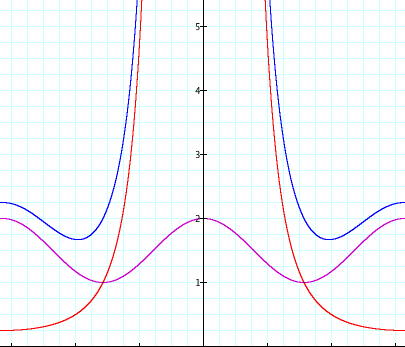
\includegraphics[scale=0.4]{differential-cross-section}
	\caption{Differential cross-section on $\Theta$ qualitatively. Red: t-channel, violet: s-channel, blue: s-channel + t-channel}
	\label{fig:diff-cross-section}
\end{figure}
For s-channel: $\frac{d\sigma}{d\Omega} \propto 1 + \cos^2{\Theta}$ (for big $Theta$)
\newline
For t-channel: $\frac{d\sigma}{d\Omega} \propto (1 - \cos{\Theta})^{-2}$ (for small $Theta$)

\subsection{Forward-Backward Asymmetry}
Based on equation (2.18)
\begin{tabular}{ |p{3cm}||p{2cm}|p{2cm}|p{2cm}|  }
 \hline
 \multicolumn{4}{|c|}{Forward-Bckward asymmetry} \\
 \hline
 $\sqrt{s}$ / $\sin^2(\theta_W)$ & 0.21 & 0.23 & 0.25 \\
 \hline
   89.225 GeV & 0.547 & 0.321 & 0.285  \\
   91.225 GeV & 0.530 & 0.407 & 0.284  \\
   93.225 GeV & 0.515 & 0.480 & 0.284  \\
  \hline
\end{tabular}
\begin{figure}[H]
	\centering
	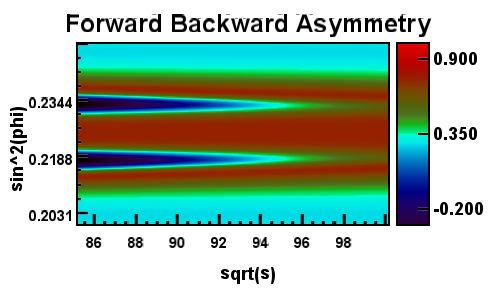
\includegraphics[scale=0.6]{forward_backward_symmetry}
	\caption{Forward-Bckward asymmetry}
	\label{fig:for-back-asy}
\end{figure}

\section{Analyzing Data}

\subsection{Pure Events}
For the $e^+, e^-$ detection we have to apply a cut for the $-0.71 \leq \cos(\theta) \leq 0.65$ and  $-0.925 \leq \cos(\theta) \leq -0.85$ due to a problem in the detector.
\newline

\subsubsection{Z->$e^+, e^-$}
\begin{itemize}  
\item All energy in Ecal
\item None in Hcal
\item 2 charged traces
\item Momentum of charged traces around $Z_M$
\end{itemize}

\subsubsection{Z->$\mu^+, \mu^-$}
\begin{itemize}  
\item None in Ecal
\item Very little in Hcal
\item 2 charged traces
\item Momentum of charged traces around $Z_M$
\item For $\cos(\theta) leq -0.7$ and $\cos(\theta) geq 0.7$ the slope for differential cross-section is not as expected. Thus cut it.
\end{itemize}

\subsubsection{Z->$\tau^+, \tau^-$}
asd

\subsection{Seperating t-channel for $e^+ e^-$}
We are looking for a cut to remove all t-channel events. Therefore we define
\begin{equation}
\frac{T}{T+S} \leq 0.05
\end{equation}
where  $T=a(1-\cos{\theta})^{-2}$  and $S=b(1+\cos^2{\theta})$. And write


\begin{equation}
\frac{dN}{d\cos\theta} = \frac{a}{(1-\cos\theta)^2}+b(1+\cos^2\theta)
\end{equation}
Integrate $\cos\theta$
\begin{equation}
\int dN = \frac{a}{1-\cos\theta} + b\left(\cos\theta+\frac{1}{3}\cos^3\theta\right)
\end{equation}
We obtain detector errors outside $cos\theta \in [-0.7,0.7]$. To solve the equation for a and b we create 2 equations by split around $\cos\theta=0$.
\begin{equation}
\begin{split}
11786 &= a(\frac{1}{1-0.7}-1)+b(0,7+\frac{1}{3}0.7^3) \\
9620 &= a(1-\frac{1}{1+0.7})+b(0,7+\frac{1}{3}0.7^3) \\
\end{split}
\end{equation}
So we get
\begin{equation}
\begin{split}
11786 &= (2+\frac{1}{3})a+0,813433b \\
9620 &= 0,4117647a+ 0,813433b \\
\end{split}
\end{equation}
So $a=1127,2$ and $b=9155,857$.
We want $\frac{T}{T+S} \leq 0.05$ so we need to solve 
\begin{equation}
\frac{a}{(1-\cos\theta)^2}\frac{1}{\frac{a}{(1-\cos\theta)^2}+b(1+\cos^2\theta))} \leq 0.05 \iff \cos\theta \leq -0.188342
\end{equation}

To get true number of s-channel events we now integrate over the whole interval 
\begin{equation}
N_s = b\int_{-1}^1 d\cos\theta (1+\cos^2\theta) = \frac{8}{3}b = 24413
\end{equation}

\subsection{Create efficiency matrix}
We create efficiency matrix where each element is given by 
\begin{equation}
\epsilon = \frac{N_{cut}}{N_{true}}
\end{equation}
Thus performing the cuts to data set XX we could create the following matrix
\begin{equation}
\epsilon=\begin{pmatrix}
   2.86\cdot 10^{-01} & 1.0\cdot 10^{-05} & 0 & 0 \\
   0 & 9.18\cdot 10^{-01} & 5.77\cdot 10^{-03} & 0 \\
   3.03\cdot 10^{-03} & 9.13\cdot 10^{-03} & 7.93\cdot 10^{-01} & 4.05\cdot 10^{-03} \\
   1.02\cdot 10^{-03} & 0 & 1.2\cdot 10^{-02} & 9.95\cdot 10^{-01} \\
\end{pmatrix}
\end{equation}
To find filter background and find $N_{true}$ we need to solve the following equation
\begin{equation}
N_{obs} = \epsilon N_{true}
\end{equation}
Multiply left side with inverse efficiency matrix we get
\begin{equation}
\epsilon^{-1} N_{obs} = N_{true}
\end{equation}
with inverse efficiency matrix
\begin{equation}
\epsilon^{-1}=\begin{pmatrix}
   3.5 & -3.81\cdot 10^{-05} & 2.77\cdot 10^{-07} & -1.13\cdot 10^{-09} \\
   8.39\cdot 10^{-05} & 1.09 & -7.92\cdot 10^{-03} & 3.23\cdot 10^{-05} \\
   -1.33\cdot 10^{-02} & -1.25\cdot 10^{-02} & 1.26 & -5.13\cdot 10^{-03} \\
   -3.43\cdot 10^{-03} & 1.51\cdot 10^{-04} & -1.52\cdot 10^{-02} & 1.01 \\
\end{pmatrix}
\end{equation}
The error of efficiency matrix is given by
\begin{equation}
\Delta \epsilon = \sqrt{\frac{\epsilon(1-\epsilon)}{N}}
\end{equation}
Using $\epsilon\Delta\epsilon^{-1}+\Delta\epsilon\epsilon^{-1}=0$ we get error for inverse efficiency matrix:
\begin{equation}
\Delta\epsilon^{-1} = -\epsilon^{-1}\Delta\epsilon\epsilon^{-1} = \begin{pmatrix}
   -3.55 \cdot 10^{-02} & 4.24 \cdot 10^{-07} & 1.08 \cdot 10^{-08} & -9.96 \cdot 10^{-11} \\
   1.43 \cdot 10^{-05} & -1.06 \cdot 10^{-03} & -3.9 \cdot 10^{-04} & 3.18 \cdot 10^{-06} \\
   -1.6 \cdot 10^{-03} & -3.78 \cdot 10^{-04} & -2.21 \cdot 10^{-03} & -2.43 \cdot 10^{-04} \\
   -6.42 \cdot 10^{-04} & 9.57 \cdot 10^{-06} & -4.77 \cdot 10^{-04} & -1.97 \cdot 10^{-04} \\
\end{pmatrix}
\end{equation}

Apply the filters we used within monte carlo simulation we could find the total number of observed events for each $\sqrt{s} \in \{...\}$:
\begin{equation}
N_{obs}=\begin{pmatrix}
   2.0\cdot 10^{+01} & 9.0\cdot 10^{+01} & 1.0\cdot 10^{+02} & 2.0\cdot 10^{+03} \\
   8.0\cdot 10^{+01} & 3.0\cdot 10^{+02} & 3.0\cdot 10^{+02} & 7.0\cdot 10^{+03} \\
   9.0\cdot 10^{+01} & 4.0\cdot 10^{+02} & 3.0\cdot 10^{+02} & 9.0\cdot 10^{+03} \\
   6.0\cdot 10^{+02} & 3.0\cdot 10^{+03} & 2.0\cdot 10^{+03} & 7.0\cdot 10^{+04} \\
   1.0\cdot 10^{+02} & 6.0\cdot 10^{+02} & 5.0\cdot 10^{+02} & 1.0\cdot 10^{+04} \\
   4.0\cdot 10^{+01} & 3.0\cdot 10^{+02} & 3.0\cdot 10^{+02} & 6.0\cdot 10^{+03} \\
   6.0\cdot 10^{+01} & 3.0\cdot 10^{+02} & 3.0\cdot 10^{+02} & 7.0\cdot 10^{+03} \\
\end{pmatrix}
\end{equation}
Thus we get using inverse efficiency matrix
\begin{equation}
N_{true} = (\epsilon^{-1}N_{obs}^T)^T = \begin{pmatrix}
   6.995\cdot 10^{+01} & 1.006\cdot 10^{+02} & 1.08\cdot 10^{+02} & 2.512\cdot 10^{+03} \\
   2.833\cdot 10^{+02} & 3.053\cdot 10^{+02} & 2.966\cdot 10^{+02} & 6.682\cdot 10^{+03} \\
   3.183\cdot 10^{+02} & 4.214\cdot 10^{+02} & 3.838\cdot 10^{+02} & 8.812\cdot 10^{+03} \\
   2.207\cdot 10^{+03} & 3.12\cdot 10^{+03} & 2.635\cdot 10^{+03} & 6.718\cdot 10^{+04} \\
   3.987\cdot 10^{+02} & 6.252\cdot 10^{+02} & 5.346\cdot 10^{+02} & 1.306\cdot 10^{+04} \\
   1.294\cdot 10^{+02} & 2.847\cdot 10^{+02} & 2.805\cdot 10^{+02} & 6.287\cdot 10^{+03} \\
   1.959\cdot 10^{+02} & 3.163\cdot 10^{+02} & 2.812\cdot 10^{+02} & 7.016\cdot 10^{+03} \\
\end{pmatrix}
\end{equation}
with error of 
\begin{equation}
\Delta N_{true} = \begin{pmatrix}
   -7.095\cdot 10^{-01} & -1.284\cdot 10^{-01} & -8.901\cdot 10^{-01} & -5.511\cdot 10^{-01} \\
   -2.873 & -3.809\cdot 10^{-01} & -2.443 & -1.487 \\
   -3.228 & -5.185\cdot 10^{-01} & -3.19 & -1.948 \\
   -2.238\cdot 10^{+01} & -3.771 & -2.367\cdot 10^{+01} & -1.47\cdot 10^{+01} \\
   -4.044 & -7.586\cdot 10^{-01} & -4.633 & -2.861 \\
   -1.313 & -3.568\cdot 10^{-01} & -2.236 & -1.375 \\
   -1.987 & -3.866\cdot 10^{-01} & -2.463 & -1.531 \\
\end{pmatrix}
\end{equation}
Next we calculate crossection by using equation (S-3.3):
\begin{equation}
\frac{dN}{dt} = \mathcal{L}\sigma
\label{eq:cs}
\end{equation}
Using the following matrix for Strahlungskorrektur from table 5.5
\begin{equation}
\Lambda = \begin{pmatrix}
   9.0\cdot 10^{-02} & 9.0\cdot 10^{-02} & 9.0\cdot 10^{-02} & 2.0 \\
   2.0\cdot 10^{-01} & 2.0\cdot 10^{-01} & 2.0\cdot 10^{-01} & 4.3 \\
   3.6\cdot 10^{-01} & 3.6\cdot 10^{-01} & 3.6\cdot 10^{-01} & 7.7 \\
   5.2\cdot 10^{-01} & 5.2\cdot 10^{-01} & 5.2\cdot 10^{-01} & 1.08\cdot 10^{+01} \\
   2.2\cdot 10^{-01} & 2.2\cdot 10^{-01} & 2.2\cdot 10^{-01} & 4.7 \\
   -1.0\cdot 10^{-02} & -1.0\cdot 10^{-02} & -1.0\cdot 10^{-02} & -2.0\cdot 10^{-01} \\
   -8.0\cdot 10^{-02} & -8.0\cdot 10^{-02} & -8.0\cdot 10^{-02} & -1.6 \\
\end{pmatrix}
\end{equation}
And the following Luminosities given by table 5.6:
\begin{equation}
\mathcal{L}dt = \begin{pmatrix}
   4.6398\cdot 10^{+02} \\
   6.6752\cdot 10^{+02} \\
   4.8676\cdot 10^{+02} \\
   2.2466\cdot 10^{+03} \\
   5.3591\cdot 10^{+02} \\
   4.506\cdot 10^{+02} \\
   7.097\cdot 10^{+02} \\
\end{pmatrix}
\end{equation}
We calculate the crossection for each element $\sigma_{ij} = N_{true,ij}/(\mathcal{L}dt)_i-\Lambda_{ij}$:
\begin{equation}
\sigma = \begin{pmatrix}
   1.33105\cdot 10^{-01} & 2.9044\cdot 10^{-01} & 2.99061\cdot 10^{-01} & 7.38817 \\
   3.21344\cdot 10^{-01} & 6.22457\cdot 10^{-01} & 5.98488\cdot 10^{-01} & 1.42622\cdot 10^{+01} \\
   5.46949\cdot 10^{-01} & 1.15915 & 1.06876 & 2.57169\cdot 10^{+01} \\
   8.00873\cdot 10^{-01} & 1.80151 & 1.58741 & 4.05623\cdot 10^{+01} \\
   4.32723\cdot 10^{-01} & 1.29668 & 1.12314 & 2.89486\cdot 10^{+01} \\
   7.21127\cdot 10^{-02} & 5.73666\cdot 10^{-01} & 5.47035\cdot 10^{-01} & 1.36859\cdot 10^{+01} \\
   -1.0932\cdot 10^{-03} & 3.31443\cdot 10^{-01} & 2.79308\cdot 10^{-01} & 8.23799 \\
\end{pmatrix}
\end{equation}

The error of crossection in eq (\ref{eq:cs}) is given by
\begin{equation}
\Delta\sigma = \sqrt{\left(\frac{\partial\sigma}{\partial N_{True}}\Delta N_{True}\right)^2+
\left(\frac{\partial\sigma}{\partial (\mathcal{L}dt)}\Delta{\mathcal{L}dt}\right)^2} = \sqrt{\left(\frac{1}{\mathcal{L}dt}\Delta N_{True}\right)^2
+\left(-\frac{N_{True}}{(\mathcal{L}dt)^2}\Delta\mathcal{L}dt\right)^2}
\end{equation}
Where the error of $\mathcal{L}dt$ is given by
\begin{equation}
\Delta\mathcal{L}dt = \pm \begin{pmatrix}
   4.249604 \\
   5.691792 \\
   4.454466 \\
   16.43293 \\
   4.848926 \\
   4.276552 \\
   6.104764 \\
\end{pmatrix} [nb^{-1}]
\end{equation}
Finally we get
\begin{equation}
\Delta\sigma=\begin{pmatrix}
   2.0603\cdot 10^{-03} & 2.0057\cdot 10^{-03} & 2.8681\cdot 10^{-03} & 4.96\cdot 10^{-02} \\
   5.6236\cdot 10^{-03} & 3.9419\cdot 10^{-03} & 5.2671\cdot 10^{-03} & 8.5376\cdot 10^{-02} \\
   8.9322\cdot 10^{-03} & 7.9929\cdot 10^{-03} & 9.747\cdot 10^{-03} & 1.6571\cdot 10^{-01} \\
   1.2284\cdot 10^{-02} & 1.0296\cdot 10^{-02} & 1.3589\cdot 10^{-02} & 2.1885\cdot 10^{-01} \\
   1.0112\cdot 10^{-02} & 1.065\cdot 10^{-02} & 1.2499\cdot 10^{-02} & 2.2052\cdot 10^{-01} \\
   3.9891\cdot 10^{-03} & 6.0496\cdot 10^{-03} & 7.716\cdot 10^{-03} & 1.3245\cdot 10^{-01} \\
   3.6702\cdot 10^{-03} & 3.8727\cdot 10^{-03} & 4.8643\cdot 10^{-03} & 8.506\cdot 10^{-02} \\
\end{pmatrix}
\end{equation}






\pagebreak
\nocite{*}
\printbibliography



\end{document}